% Chapter Template

\chapter{Introduction} % Main chapter title

\label{ch:introduction} % Change X to a consecutive number; for referencing this chapter elsewhere, use \ref{ChapterX}

%Surface normal is an important property of a surface with many applications, like surface reconstruction, shadings generation and other visual effects. However, the calculation of surface normal in many tasks is not as straightforward as simply the cross-product of two plane vectors. Especially in the task of real-world object digitalization, the surface is usually hardly to be mathematically described in equations due to the elaborate details on the objects. 
%
%Instead, it is common to infer it from the object point cloud. The point cloud records a great number of point positions on the object surface. These numbers of points altogether, are called point cloud, which is a memory economical solution to describe the shape of the object surface. They contains the geometry information of the surface, thus can be used for surface normal inference.
%




%
%Apart from this, due to the application scenarios, the working principle of scanners are various, which consequently produce point cloud structures in different forms. For the scanners without positions recording, the point cloud is unstructured. In this case, every 3D point can be captured by different capture position, and neighbors are not defined by capture time. It increases the difficulty and computation for the neighbor based normal inference approaches.  Furthermore, since the lack of inherent structure, the normal can hardly be inferred by the parallel approaches. 
%
%Thus getting a structured point cloud from a calibrated scanner is a much more convenient choice. One solution is the depth camera. It captures the RGB-D images of the object, which includes the standard RGB image with depth information of each pixel. Based on the calibrated camera, it is easy to acquire the structured surface point cloud from depth map and camera matrix. Furthermore, the point cloud is mapped directly based on the 2D depth map with the same capture position. which keeps the neighbor information of each point.  It is identical to the corresponding pixel in the 2D depth map. This provides a better view for the normal inference task since the neighbor information can be considered as a reference. 
%
%Besides geometry based approach, photometric stereo based approach using a set of light sources with knowing positions to separately project lights on the object, the surface normal can be calculated from the captured images and the known light directions. It is different from geometry based approach since no surface position is required. However, it usually require many different light positions to acquire a good performance \cite{spline-net} \cite{CNN-PS}, which raise the complexity for the data collection.
%
%Actually, the depth camera is able to acquire both geometry information like depth map as well as the images as photometric information. They are usually acquired at the same time when we collect the data. This inspired us to utilize the both depth map and image information to infer the surface map in order to find a more practical and more accurate approach that integrate two kinds of information and consequently improved surface normal inference.
%
%
%Deep learning based methods provides multiple possible solutions for the challenges mentioned above. First, to deal with the noised input, deep learning based methods already have the solution for the similar tasks like image inpainting and depth density enhancement, which base on the noised image as input to predict the clean and fully dense output with or without original meanings. Therefore, it can be a help for noise in the depth map. Besides, the network of deep learning model can also handle the structured point cloud as a single input and infer the corresponding normal all together, which is very time economical comparing to the approaches like neighbor based methods. In addition, the multi-stages training architectures provide a way to consider both depth map and texture image as the input to predict the surface normals, which not only consider the point cloud but also the add the lambertian reflection as a further constraint.
%
%Unfortunately, in the actual situation, the depth maps captured by the sensors are only semi-dense, which is mainly caused by. Consequently, it disrupts the robustness of the normal inference methods. Median filters can be used for the sparse missing pixels, however, for the case of huge missing holes in the depth map, it produces just a paltry result. Thus a reasonable guess is required for missing areas.
%
%
%In this work, we focus on the normal inference based on a semi-dense depth map with RGB image using deep learning based approaches. Specifically, the missing pixels in the depth map is filled up by the gated convolution and propagate in a customized UNet with skipping connections. The output of the training model is directly the surface normal corresponding the input depth map. The grayscale image is used to further improve the estimation accuracy. 
%For the training work, a dataset named “synthetic50-5” is created including 55 high resolution point clouds from internet, as shown in Appendix A. The point clouds provide with the high accurate normals, which can be used as the ground truth of the training work. Most of the models have elaborate details with high curvatures but also contain smooth surfaces. The trained model is evaluated on both synthetic dataset as well as the real dataset captured from RGB-D cameras. A series of metrics have been used for qualitative evaluation. The model is shown to achieve a remarkably better prediction accuracy at a low computational cost compared to the standard approaches for semi-dense point clouds.  

%% main problem, introduce deep learning, UNet
In 3D computer vision tasks, the \textit{point cloud} ( i.e. a great number of point positions on the object surface, these numbers of points altogether, are called point cloud) is a common input data to describe the object surface. Based on the geometry information containing in the point cloud, we can acquire the corresponding surface normal, which is an importance features in computer vision, which can be further used for  surface reconstruction, shadings generation and other visual effects. A common approach to acquire the surface normal from point cloud is the optimization approach which consider the neighbor points in the same plane and calculate the plane normal. However, for the single input data with only one shot recording, like the depth camera, the acquired point cloud is converted from depth map. But due to the  optical noises and the reflections in dark and shinny areas of the object surface, the depth map is usually semi-dense only. Thus it limited the neighbor based approach since the missing data leads to less neighbors of each points. However, recent advances in image inpainting areas have motivated researchers to recover the missing regions in the input data using deep neural networks and achieves a good performance. For example, \cite{gconv} uses a gated convolution network to inpaint a custom removed areas in the images. \cite{nconv} uses normalized convolution network to enhance semi-dense depth map to fully dense depth map. Either work takes in-complete input data and mends it to fully dense output. Thus a deep learning based approach can be a way to deal with the semi-dense depth map input for surface normal estimation task.

\begin{figure}[h!]
	\centering
	{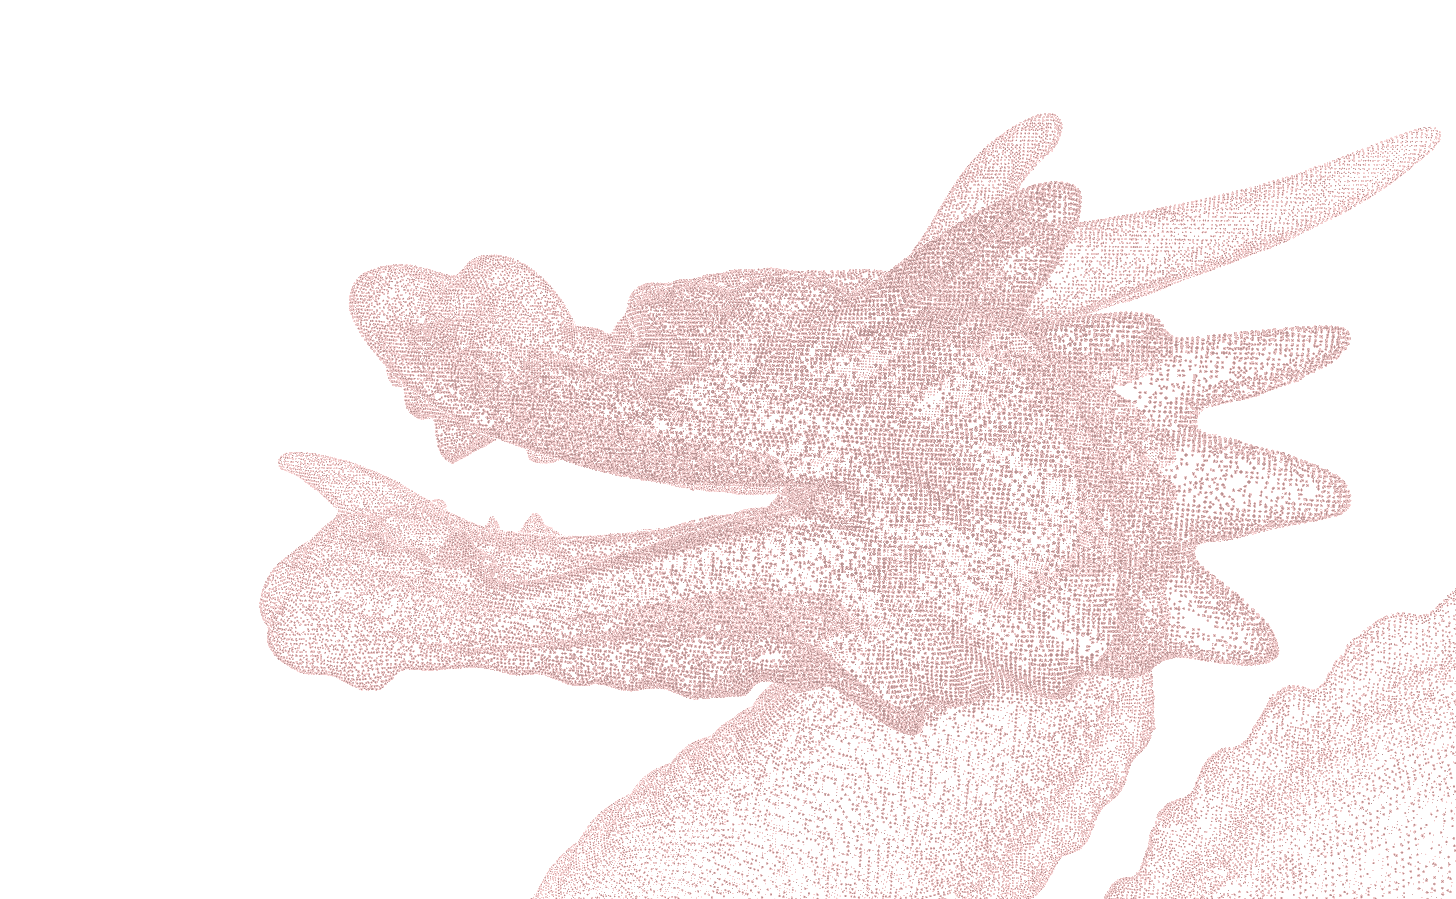
\includegraphics[width=.45\textwidth]{./Figures/point-cloud.png}}
	{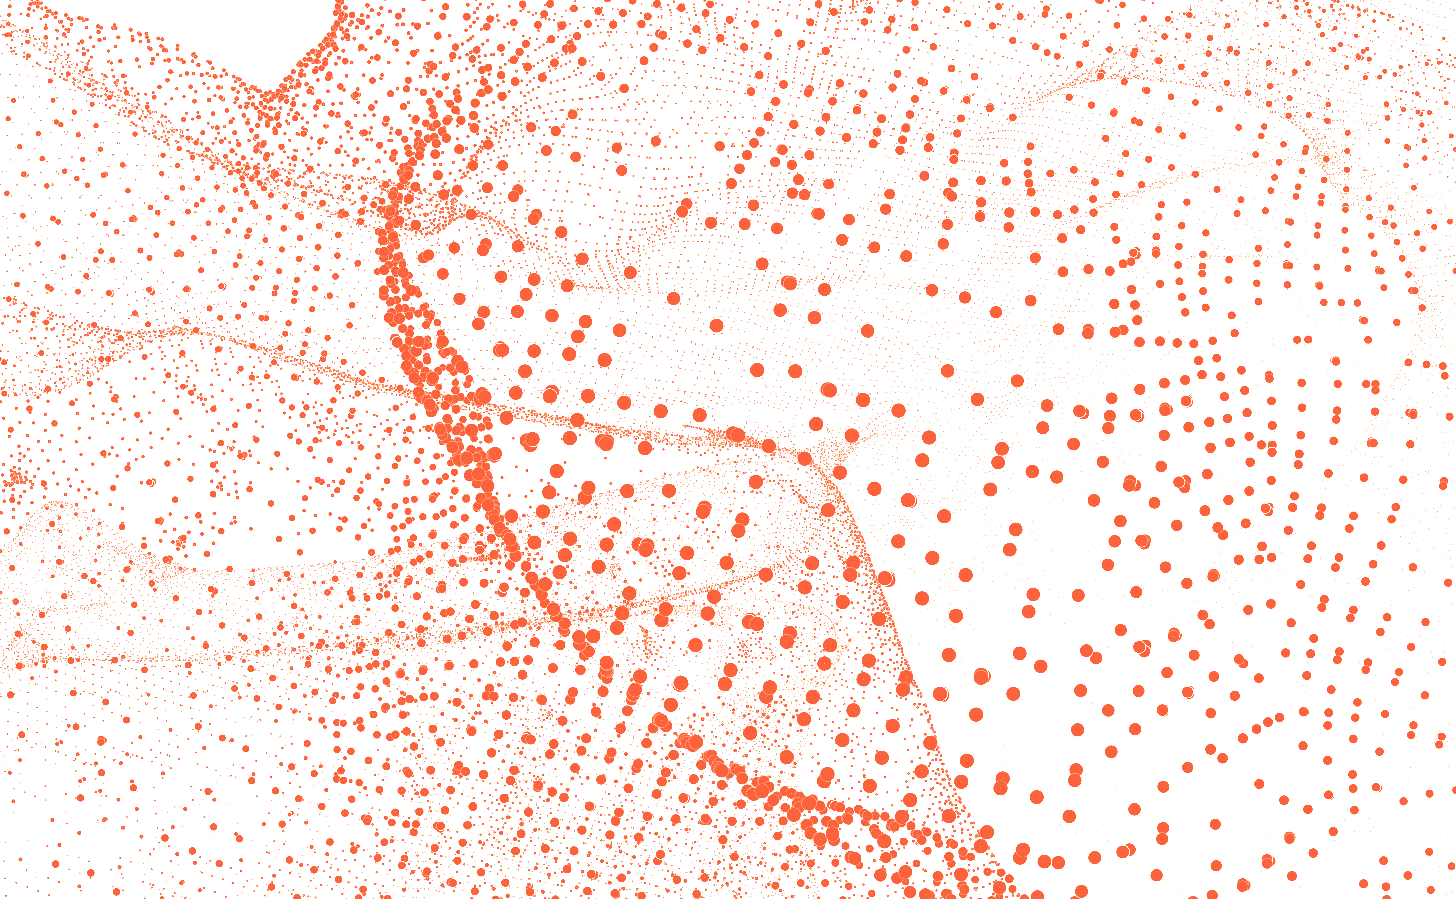
\includegraphics[width=.45\textwidth]{./Figures/point-cloud-zoom-in.png}}
	\decoRule
	\caption{Left: A piece of point cloud of the dragon object. Right: Zoom in of the point cloud.}
	\label{fig:point-cloud}
\end{figure}

%% introduce photometric stereo
Photometric stereo is another approach in computer vision which can be used for surface normal estimation, where the normals are inferred from appearance variations under multiple illuminations. The relative methods are typically solve the least square problem based on the pointwise image formation model.\cite{SFS} and based on the Bidirectional Reflectance Distribution Function (BRDF). While BRDF based model generally cannot account the global illumination effects and this is usually unavoidable problem due to the light interactions and difficult traced mathematically.

%% papers contribution, main work
Both directions mentioned above have been widely researched using deep learning approaches. However, the approach that takes both geometry and illuminated information together into account for normal estimation remains impoverishment. We present a deep learning based approach takes both geometry and photometric information into account for normal inference. For a practical reason, we consider only 1 illuminated image based on the calibrated camera and takes semi-dense point cloud as input data. To achieve this goal, we will mainly take the geometry information into consideration and take the photometric information as a supplementary.

%% introduce the network, trip-net, dataset
One of our challenge is to apply the semi-dense input data to the neural network in a image-wise way. UNet is a good network applying for computer vision task with up-sampling requirement. We modified it with gated activation unit called \textit{gated convolution layer (gconv)} to handle semi-dense input data. Another challenge is to merge the different input data feature maps together to cooperatively improved surface normal inference task. We propose a $ multi-fusion $ scheme for integration on separate feature map extractors. We will show that this multi-fusion design can be taken advantages of combination of different input data types and improved surface normal inference performance. To train our network, we create a synthetic RGB-D image dataset by utilizing one light source illumination and one ambient light illumination to simulate application scenarios. To simulate depth maps in real world, we applied uniform distributed drop-out noise to the input data with a control parameter for noise density.

%% experiments
We trained our approach on our proposed synthetic dataset ``synthetic-50-5" and evaluate it on 6 different metrics. We compare our approach against the geometry information based approach based on the similar network architecture and show that our calibrated illuminated RGB-D image based approach further improved normal accuracy. We also applied our model on real dataset and compare with the optimization based approach.

The structure of the thesis is as follows, Chapter 1 is the introduction of the whole work. Chapter 2 briefly discusses the related work about normal inference. Chapter 3 is the main approaches of this work. Chapter 4 introduces the created dataset for the training work. Chapter 5 is the description of the experiments and the evaluation of the models. Chapter 6 is the conclusion of the whole thesis.



